        %%******************************************%%
        %%                                          %%
        %%        Modello di tesi di laurea         %%
        %%            di Andrea Giraldin            %%
        %%                                          %%
        %%             2 novembre 2012              %%
        %%                                          %%
        %%******************************************%%

\begin{document}
    \frontmatter
    \begin{titlepage}
    \begin{center}
        \begin{LARGE}
            \textbf{\myUni}\\
        \end{LARGE}

        \vspace{10pt}

        \begin{Large}
            \textsc{\myDepartment}\\
        \end{Large}

        \vspace{10pt}

        \begin{large}
            \textsc{\myFaculty}\\
        \end{large}

        \vspace{30pt}
        \begin{figure}[htbp]
            \centering
            
\includegraphics[height=6cm]{unipd-logo}
        \end{figure}
        \vspace{30pt}

        \begin{LARGE}
            \textbf{\myTitle}\\
        \end{LARGE}

        \vspace{10pt}

        \begin{large}
            \textsl{\myDegree}\\
        \end{large}

        \vspace{40pt}

        \begin{large}
            \begin{flushleft}
                \textit{Relatore}\\
                \vspace{5pt}
                \profTitle\ \myProf
            \end{flushleft}

            % You can tweak the spacing to have professor and student names on the same line
            % useful if the page is broken by a long thesis title and you need more space
            % \vspace{-52pt}

            \begin{flushright}
                \textit{Laureando}\\
                \vspace{5pt}
                \myName
            \end{flushright}
        \end{large}

        \vspace{40pt}

        \line(1, 0){338} \\
        \begin{normalsize}
            \textsc{Anno Accademico \myAA}
        \end{normalsize}
    \end{center}
\end{titlepage}

    \clearpage
\phantomsection
\thispagestyle{empty}

\hfill
\vfill

\noindent\myName: \textit{\myTitle,}
\myDegree,
\textcopyright\ \myTime.

    \cleardoublepage
\phantomsection
\thispagestyle{empty}
\pdfbookmark{Dedica}{Dedica}

\vspace*{3cm}

% \begin{center}
%     Lorem ipsum dolor sit amet, consectetuer adipiscing elit. \\ \medskip
%     --- Oscar Wilde
% \end{center}

% \medskip

% \begin{center}
%     Dedicato a ...
% \end{center}

    \cleardoublepage
\phantomsection
\pdfbookmark{Sommario}{Sommario}
\begingroup
\let\clearpage\relax
\let\cleardoublepage\relax
\let\cleardoublepage\relax

\chapter*{Sommario}

Il presente documento descrive il lavoro svolto durante il periodo di stage, della durata di circa trecento ore, dal laureando Pinco Pallino presso l'azienda Azienda S.p.A.
Gli obbiettivi da raggiungere erano molteplici.\\
In primo luogo era richiesto lo sviluppo di ...
In secondo luogo era richiesta l'implementazione di un ...
Tale framework permette di registrare gli eventi di un controllore programmabile, quali segnali applicati
Terzo ed ultimo obbiettivo era l'integrazione ...

%\vfill

%\selectlanguage{english}
%\pdfbookmark{Abstract}{Abstract}
%\chapter*{Abstract}

%\selectlanguage{italian}

\endgroup

\vfill

    \cleardoublepage
\phantomsection
\pdfbookmark{Ringraziamenti}{ringraziamenti}

% \begin{flushright}{
%     \slshape
%     ``Life is really simple, but we insist on making it complicated''} \\
%     \medskip
%     --- Confucius
% \end{flushright}


\bigskip

\begingroup
\let\clearpage\relax
\let\cleardoublepage\relax
\let\cleardoublepage\relax

\chapter*{Ringraziamenti}

\noindent \textit{Innanzitutto, vorrei esprimere la mia gratitudine alla Prof.ssa \myProf, relatore della mia tesi, per l'aiuto e il sostegno fornitomi durante la stesura del lavoro.}\\

\noindent \textit{Desidero ringraziare con affetto i miei genitori e i miei nonni per il sostegno, il grande aiuto e per essermi stati vicini in ogni momento durante gli anni di studio.}\\

\noindent \textit{Desidero ringraziare Marco, Luigi, Samuel, Nicola e Andrea per il loro prezioso sostegno durante il mio percorso di laurea. La vostra amicizia, incoraggiamento e presenza costante sono stati fondamentali per il mio successo accademico. Sono grato di avervi avuto al mio fianco e custodirò i nostri momenti con affetto. Grazie di cuore, cari amici.}\\

\noindent \textit{Grazie, Sara, per essere stata il mio sostegno durante il mio percorso di laurea. Il tuo amore e la tua comprensione sono stati fondamentali. Ti sono grato di averti al mio fianco. Ti amo.}\\

\noindent \textit{Infine, vorrei ringraziare tutto il team di AdMaioraStudio per avermi guidato e supportato durante il periodo di stage}\\

% \noindent \textit{Ho desiderio di ringraziare poi i miei amici per tutti i bellissimi anni passati insieme e le mille avventure vissute.}\\
\bigskip

\noindent\textit{\myLocation, \myTime}
\hfill \myName

\endgroup

    \cleardoublepage
\pdfbookmark{\contentsname}{tableofcontents}
\setcounter{tocdepth}{2}
\tableofcontents
%\markboth{\contentsname}{\contentsname}
\clearpage

\begingroup
    \let\clearpage\relax
    \let\cleardoublepage\relax
    \let\cleardoublepage\relax

    % Figures list
    \phantomsection
    \pdfbookmark{\listfigurename}{lof}
    \listoffigures

    \vspace*{8ex}

    % Tables list
    \phantomsection
    \pdfbookmark{\listtablename}{lot}
    \listoftables

    \vspace*{8ex}
\endgroup

\cleardoublepage

    \cleardoublepage

    \mainmatter
    \chapter{Introduzione}
\label{cap:introduzione}

% Introduzione al contesto applicativo.\\

% \noindent Esempio di utilizzo di un termine nel glossario \\
% \gls{api}. \\

% \noindent Esempio di citazione in linea \\
% \cite{site:agile-manifesto}. \\

% \noindent Esempio di citazione nel pie' di pagina \\
% citazione\footcite{womak:lean-thinking} \\
\section{L'idea}

Nell'attuale panorama delle fiere e degli eventi commerciali, le aziende partecipanti hanno manifestato un crescente interesse nella promozione innovativa
dei propri prodotti. Attualmente, essa avviene principalmente attraverso la distribuzione di materiale pubblicitario, come brochure, volantini e cataloghi, 
lasciando al visitatore il compito di informarsi autonomamente sui prodotti offerti dai vari espositori.\\
In questa tesi verrà descritto lo sviluppo di una WebApp attraverso la quale gli espositori avranno la possibilità di caricare i propri video
relativi ai prodotti esposti, rendendoli successivamente disponibili per la riproduzione on-demand da parte dei visitatori.
L'idea rappresenta un passo avanti verso l'innovazione della promozione dei prodotti nelle fiere, perché offre ai partecipanti un'esperienza interattiva 
e coinvolgente. \\

\section{Descrizione dello stage}

L'azienda ha manifestato l'esigenza di sviluppare un Proof of Concept (PoC) per la realizzazione di una WebApp che permetta agli espositori di caricare i propri video relativi ai prodotti esposti, e li renda disponibili per la riproduzione on-demand da parte dei visitatori.\\
L'idea è quella di realizzare un prodotto che possa essere utilizzato in occasione di fiere ed eventi commerciali.\\
L'applicazione è stata sviluppata utilizzando come linguaggio di backend C\texttt{\#}~\footnote{\url{https://learn.microsoft.com/it-it/dotnet/csharp/}}, per lo sviluppo del frontend il framework JavaScript React~\footnote{\url{https://reactjs.org/}}  ,
mentre per la gestione dell'archiviazione e streaming dei video sono stati utilizzati i servizi di Microsoft Azure: Media Service, Account Storage, SQL Server e App Service.~\footnote{\url{https://azure.microsoft.com/}}\\
L'obbiettivo principiale di questo PoC, è stato quello di studiare e verificare la fattibilità di un prodotto di questo tipo.\\
\section{L'azienda}

Ad Maiora Studio è una software house nata nel 2013 per operare nel campo del mobile e che negli anni si è specializzata anche nello sviluppo di software.~\footnote{\url{https://admaiorastudio.com/}}\\
La sua mission è centrata sull'attenzione verso i clienti e lo sviluppo di software moderni, scalabili e progettati ad hoc per soddisfare le loro esigenze. \\
I prodotti sviluppati da Ad Maiora Studio si basano sulle più recenti tecnologie, integrano componenti e librerie eterogenee e pongono una forte enfasi sull'esperienza utente
 e l'interfaccia grafica.\\
L'azienda si distingue per l'approccio continuativo di assistenza ai clienti, 
garantendo un partner sempre accessibile e in grado di rispondere tempestivamente alle richieste. \\
Ad Maiora Studio si concentra principalmente su piccole e medie imprese operanti nei settori industriale e dei servizi, incoraggiandole a intraprendere un percorso di modernizzazione
 iniziando dal software.\\
L'obiettivo è supportare efficacemente l'adattamento alle mutevoli esigenze di mercato e di business, fornendo strumenti innovativi e personalizzati, che rappresentano il cuore dell'attività di Ad Maiora Studio.\\
Grazie alla competenza Full Stack del team di sviluppatori, l'azienda è in grado di realizzare ogni tipo di software, 
coprendo l'intero processo di sviluppo, dalla progettazione all'implementazione.\\
La qualità delle soluzioni software offerte è sempre un punto focale, al fine di soddisfare appieno le aspettative dei clienti e garantire il massimo risultato.



\section{Struttura della tesi}

\begin{description}

    \item[{\hyperref[cap:introduzione]{Il primo capitolo}}] introduce l'idea del progetto, la descrizione dello stage e l'azienda
    \item[{\hyperref[cap:fondamentiteorici]{Il secondo capitolo}}] descrive i fondamenti teorici alla base dello streaming video e le tecnologie utilizzate per la realizzazione del PoC
    
    \item[{\hyperref[cap:analisi-requisiti]{Il terzo capitolo}}] descrive gli obiettivi obbligatori, desiderabili e facoltativi, i prodotti attesi e la pianificazione del lavoro.
    
    \item[{\hyperref[cap:progettazione]{Il quarto capitolo}}] approfondisce la fase di progettazione dell'applicazione e come vengono implementate le tecnologie tra di loro per il raggiungimento degli obiettivi.
    
    \item[{\hyperref[cap:implementazione]{Il quinto capitolo}}] descrive il processo di implementazione andando nel dettaglio delle tecnologie utilizzate.
    
    \item[{\hyperref[cap:testing]{Il sesto capitolo}}] approfondisce la fase di Unit Test del backend e dei risultati ottenuti

    \item[{\hyperref[cap:analisi-costi]{Il settimo capitolo}}] descrive l'analisi dei costi effettuata per il mantenimento dell'applicazione in base al numero di utenti.

    
    \item[{\hyperref[cap:conclusioni]{L'ottavo capitolo}}] descrive il raggiungimento degli obiettivi, le conoscenze acquisite e la valutazione personale del progetto.
\end{description}


    \chapter{Descrizione dello stage}
\intro{In questo capitolo verrà descritto lo stage, partendo dalla descrizione di esso, gli obiettivi, la pianificazione, i risultati attesi ecc..}\\
\label{cap:descrizione-stage}
\section{Obiettivi}
\label{sec:obiettivi}
Seguono gli obbietti identificati nel piano di lavoro.
\subsection{Notazione}
\label{subsec:notazione}
Gli obiettivi sono cosi identificati:
\begin{itemize}
    \item \textbf{O} per gli obiettivi obbligatori;
    \item \textbf{D} per gli obiettivi desiderabili;
    \item \textbf{F} per gli obiettivi facoltativi.
\end{itemize}
\subsection{Obiettivi obbligatori}
obiettivi obbligatori:
\begin{itemize}
    \item \textbf{O1} Realizzazione del POC;
    \item \textbf{O2} Sviluppo Unit test backend;
    \item \textbf{O3} Analisi dei costi;
    \item \textbf{O4} Stesura della documentazione.
\end{itemize}
\subsection{Obiettivi desiderabili}
obiettivi desiderabili:
\begin{itemize}
    \item \textbf{D1} Analisi approfondita e comparazione di diverse architetture e sul loro impatto sui costi;
    \item \textbf{D2} Analisi dei competitor per osservare la gestione dei problemi di carico elevato.
\end{itemize}
\subsection{Obiettivi facoltativi}
obiettivi facoltativi:
\begin{itemize}
    \item \textbf{F1} Analisi dei sviluppi futuri;
    \item \textbf{F2} Realizzazione di un'interfaccia grafica, funzionale e conforme agli standard qualitativi di un'applicazione moderna.

\end{itemize}
\section{Pianificazione}
\label{sec:pianificazione}
\begin{table}[!h]
    \label{tab:ripartizione-ore}
    \begin{tabularx}{\textwidth}{|c|X|}
        \hline
        \textbf{Durata in ore} & \textbf{Descrizione dell'attività} \\\hline
        
        \textbf{80} & \textbf{Formazione sulle tecnologie} \\ \hdashline
            \multirow{2}{0cm}\\
                \textit{30} &
                \textit{Studio delle basi dello stack tecnologico utilizzato dall'azienda e dei metodi di sviluppo} \\
                \textit{50} &
                \textit{Studio e comparazione dei servizi offerti da Azure per realizzare la web app. Analisi di pro e contro dei vari servizi.} \\
        \hline
        
        \textbf{180} & \textbf{Sviluppo} \\ \hdashline 
        \multirow{3}{0cm}\\ 
        \textit{40} & 
        \textit{Realizzazione della struttura di base della web app considerando le analisi di cui sopra.} \\
        \textit{100} & 
        \textit{Implementazione di front-end, back-end e DB} \\
        \textit{80} & 
        \textit{Test, ottimizzazione, refactoring. Realizzazione di unit test.} \\
        \hline
        
        \textbf{40} & \textbf{Documentazione e Demo}  \\ \hdashline 
        \multirow{4}{0cm}\\ 
        \textit{25} & 
        \textit{Collaudo} \\
        \textit{10} & 
        \textit{Stesura documentazione finale} \\
        \textit{1} & 
        \textit{Incontro di presentazione della piattaforma con gli stakeholders} \\
        \textit{2} & 
        \textit{Live demo di tutto il lavoro di stage} \\
        \hline
        
        \textbf{Totale ore} & \multicolumn{1}{|c|}{\textbf{300}} \\\hline
        
        
    \end{tabularx}
    \caption{Tabella di ripartizione delle ore}

\end{table}
\section{Prodotti attesi}
\label{sec:prodotti-attesi}
\begin{itemize}
    \item \textbf{POC} \\
    Realizzazione di un POC funzionante che dimostri la fattibilità dell'idea proposta.
    \item \textbf{Unit test} \\
    Realizzazione completa degli unit test per il backend.\\
    \item \textbf{Analisi dei costi} \\
    Analisi dei costi simulando vari scenari di utilizzo della piattaforma.\\
    \item \textbf{Documentazione} \\
    Documentazione completa di tutte le fasi di sviluppo e analisi.
    \begin{enumerate}
        \item Lettura e documentazione \\
         Documentare le varie opzioni disponibili per lo sviluppo di un'applicazione cloud, tecniche e tecnologie utilizzate e dei loro sviluppi futuri.
        \item Sviluppo e analisi \\
        Preparazione dell'ambiente di sviluppo, sviluppo del POC e delle sue componenti.
        \item Conclusioni \\
        Documentazione completa degli artefatti sviluppati e definizione dei possibili casi d'uso.
    \end{enumerate}
\end{itemize}
\section{Risorse messe a disposizione}
\label{sec:risorse-messe-a-disposizione}
Per lo svolgimento dello stage sono state messe a disposizione le seguenti risorse:
\begin{itemize}
    \item \textbf{Account Azure DevOps} \\
    Account Azure DevOps per la gestione del progetto, delle sue attività e del versionamento del codice.
    \item \textbf{Account Azure} \\
    Account Azure per la gestione delle risorse cloud.
\end{itemize}

\section{Processo sviluppo prodotto}
Il processo di sviluppo seguirà la pianificazione descritta nella sezione \ref{sec:pianificazione} e sarà suddiviso nelle seguenti fasi:
\begin{enumerate}
    \item \textbf{Formazione} \\
    Studio delle tecnologie e dei metodi di sviluppo utilizzati dall'azienda.
    \item \textbf{Analisi} \\
    Analisi delle tecnologie e dei servizi offerti da Azure per la realizzazione del POC.
    \item \textbf{Sviluppo} \\
    Sviluppo del POC e delle sue componenti.
    \item \textbf{Collaudo} \\
    Collaudo del POC e documentazione finale.
\end{enumerate}

    \chapter{Descrizione dello stage}
\label{cap:descrizione-stage}

\intro{Breve introduzione al capitolo}\\

\section{Introduzione al progetto}

\section{Analisi preventiva dei rischi}

Durante la fase di analisi iniziale sono stati individuati alcuni possibili rischi a cui si potrà andare incontro.
Si è quindi proceduto a elaborare delle possibili soluzioni per far fronte a tali rischi.\\

\begin{risk}{Performance del simulatore hardware}
    \riskdescription{le performance del simulatore hardware e la comunicazione con questo potrebbero risultare lenti o non abbastanza buoni da causare il fallimento dei test}
    \risksolution{coinvolgimento del responsabile a capo del progetto relativo il simulatore hardware}
    \label{risk:hardware-simulator} 
\end{risk}

\section{Requisiti e obiettivi}


\section{Pianificazione}

    \chapter{Analisi dei requisiti}
\label{cap:analisi-requisiti}

\intro{Breve introduzione al capitolo}\\

\section{Casi d'uso}

Per lo studio dei casi di utilizzo del prodotto sono stati creati dei diagrammi.
I diagrammi dei casi d'uso (in inglese \emph{Use Case Diagram}) sono diagrammi di tipo \gls{uml} dedicati alla descrizione delle funzioni o servizi offerti da un sistema, così come sono percepiti e utilizzati dagli attori che interagiscono col sistema stesso.
Essendo il progetto finalizzato alla creazione di un tool per l'automazione di un processo, le interazioni da parte dell'utilizzatore devono essere ovviamente ridotte allo stretto necessario. Per questo motivo i diagrammi d'uso risultano semplici e in numero ridotto.

\begin{figure}[!h] 
    \centering 
    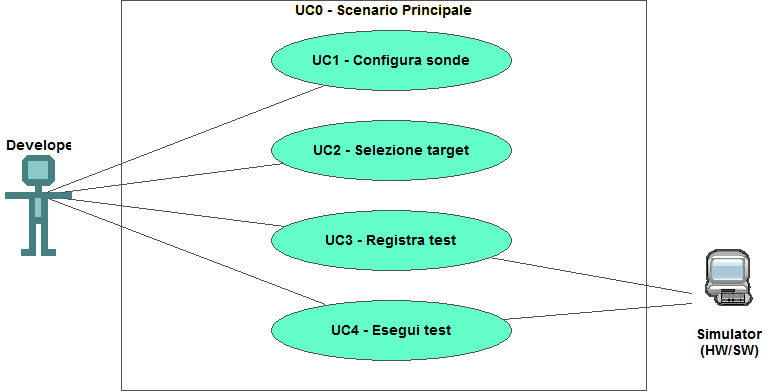
\includegraphics[width=0.9\columnwidth]{usecase/scenario-principale} 
    \caption{Use Case - UC0: Scenario principale}
\end{figure}

\begin{usecase}{0}{Scenario principale}
\usecaseactors{Sviluppatore applicativi}
\usecasepre{Lo sviluppatore è entrato nel plug-in di simulazione all'interno dell'IDE}
\usecasedesc{La finestra di simulazione mette a disposizione i comandi per configurare, registrare o eseguire un test}
\usecasepost{Il sistema è pronto per permettere una nuova interazione}
\label{uc:scenario-principale}
\end{usecase}

\section{Tracciamento dei requisiti}

Da un'attenta analisi dei requisiti e degli use case effettuata sul progetto è stata stilata la tabella che traccia i requisiti in rapporto agli use case.\\
Sono stati individuati diversi tipi di requisiti e si è quindi fatto utilizzo di un codice identificativo per distinguerli.\\
Il codice dei requisiti è così strutturato R(F/Q/V)(N/D/O) dove:
\begin{enumerate}
	\item[R =] requisito
    \item[F =] funzionale
    \item[Q =] qualitativo
    \item[V =] di vincolo
    \item[N =] obbligatorio (necessario)
    \item[D =] desiderabile
    \item[Z =] opzionale
\end{enumerate}
Nelle tabelle \ref{tab:requisiti-funzionali}, \ref{tab:requisiti-qualitativi} e \ref{tab:requisiti-vincolo} sono riassunti i requisiti e il loro tracciamento con gli use case delineati in fase di analisi.

\newpage

\begin{table}%
\caption{Tabella del tracciamento dei requisti funzionali}
\label{tab:requisiti-funzionali}
\begin{tabularx}{\textwidth}{lXl}
\hline\hline
\textbf{Requisito} & \textbf{Descrizione} & \textbf{Use Case}\\
\hline
RFN-1     & L'interfaccia permette di configurare il tipo di sonde del test & UC1 \\
\hline
\end{tabularx}
\end{table}%

\begin{table}%
\caption{Tabella del tracciamento dei requisiti qualitativi}
\label{tab:requisiti-qualitativi}
\begin{tabularx}{\textwidth}{lXl}
\hline\hline
\textbf{Requisito} & \textbf{Descrizione} & \textbf{Use Case}\\
\hline
RQD-1    & Le prestazioni del simulatore hardware deve garantire la giusta esecuzione dei test e non la generazione di falsi negativi & - \\
\hline
\end{tabularx}
\end{table}%

\begin{table}%
\caption{Tabella del tracciamento dei requisiti di vincolo}
\label{tab:requisiti-vincolo}
\begin{tabularx}{\textwidth}{lXl}
\hline\hline
\textbf{Requisito} & \textbf{Descrizione} & \textbf{Use Case}\\
\hline
RVO-1    & La libreria per l'esecuzione dei test automatici deve essere riutilizzabile & - \\
\hline
\end{tabularx}
\end{table}%

    \chapter{Progettazione e codifica}
\label{cap:progettazione-codifica}

\intro{Breve introduzione al capitolo}\\

\section{Tecnologie e strumenti}
\label{sec:tecnologie-strumenti}

Di seguito viene data una panoramica delle tecnologie e strumenti utilizzati.

\subsection*{Tecnologia 1}
Descrizione Tecnologia 1.

\subsection*{Tecnologia 2}
Descrizione Tecnologia 2

\section{Ciclo di vita del software}
\label{sec:ciclo-vita-software}

\section{Progettazione}
\label{sec:progettazione}

\subsubsection{Namespace 1} %**************************
Descrizione namespace 1.

\begin{namespacedesc}
    \classdesc{Classe 1}{Descrizione classe 1}
    \classdesc{Classe 2}{Descrizione classe 2}
\end{namespacedesc}


\section{Design Pattern utilizzati}

\section{Codifica}

    \chapter{Verifica e validazione}
\label{cap:verifica-validazione}

    \chapter{Conclusioni}
\label{cap:conclusioni}

\section{Raggiungimento degli obiettivi}
Il PoC sviluppato permette agli utenti la visualizzazione dei video e la possibilità di cambiare la qualità di visualizzazione, dà la possibilità agli espositori di caricare i video relativi ai propri prodotti e di gestirli e permette agli amministratori di gestire gli utenti, gli eventi e i video.\\
È stato sviluppato utilizzando le tecnologie richieste dall'azienda, in particolare React per il frontend, .NET Core per il backend e Azure per la gestione dei video e del database.\\
Inoltre sono stati sviluppati parzialmente gli unit test per il backend per verificare il corretto funzionamento delle funzionalità.\\
Successivamente è stata effettuata un analisi dei costi per il mantenimento dell'applicazione in base al numero di utenti utilizzatori dell'applicazione.\\
Infine è stata redatta la documentazione di resoconto finale, che descrive il lavoro svolto e i risultati ottenuti.\\
Concludendo, tutti gli obiettivi obbligatori sono stati raggiunti, tranne la realizzazione degli Unit Test completa del backend a causa di mancanza di tempo.\\
\section{Sviluppi futuri}
Il PoC sviluppato è una buona base per la realizzazione del prodotto finale, ma necessita di alcuni miglioramenti.\\
In particolare, l'aggiunta di un sistema di autenticazione per gli utenti, in modo da poter accedere all'applicazione solo se registrati, e di un sistema di autenticazione per gli espositori, in modo da poter caricare i video solo se autenticati.\\
Inoltre, sarebbe utile aggiungere un sistema di engagement per gli utenti, in modo da poter interagire con gli espositori e con gli altri utenti tramite commenti e valutazione dei prodotti.\\
Infine, è necessario aggiungere un sistema di controllo degli errori, in modo da poter gestire gli errori che possono verificarsi durante l'utilizzo dell'applicazione.\\

\section{Conoscenze acquisite}
Grazie a questa esperienza ho avuto l'opportunita di imparare nuove tecnologie come React, il framework .NET Core e il sistema di Azure, sicuramente molto utili per il mio futuro professionale. Inoltre, ho potuto approfondire le mie conoscenze in ambito di sviluppo web e di architetture software.\\
\section{Valutazione personale}
Sono molto soddisfatto del lavoro svolto, in particolare per la realizzazione del prototipo funzionante, che mi ha permesso di mettere in pratica le conoscenze acquisite durante il corso di studi e di imparare nuove tecnologie. Sicuramente il prodotto finale sarà molto utile per l'azienda presso la quale ho svolto tirocinio, in quanto ritengo sia una buona base dalla quale partire per la realizzazione del prodotto finale.\\ 
Questa esperienza ha confermato che il percorso di studi che ho scelto è quello giusto per me e mi ha approcciato verso il mondo del lavoro, che ho potuto conoscere meglio.\\

    \appendix
    \chapter{Appendice A}

\epigraph{Citazione}{Autore della citazione}


    \backmatter
    \printglossary[type=\acronymtype, title=Acronimi e abbreviazioni, toctitle=Acronimi e abbreviazioni]
    \printglossary[type=main, title=Glossario, toctitle=Glossario]

    \cleardoublepage
\chapter{Bibliografia}

\nocite{*}

% Print book bibliography
\printbibliography[heading=subbibliography,title={Riferimenti bibliografici},type=book]

% Print site bibliography
\printbibliography[heading=subbibliography,title={Siti web consultati},type=online]

\end{document}
